\documentclass[a4paper]{book}
\usepackage{a4wide}
\usepackage{makeidx}
\usepackage{fancyhdr}
\usepackage{graphicx}
\usepackage{multicol}
\usepackage{float}
\usepackage{textcomp}
\usepackage{alltt}
\usepackage{times}
\usepackage{ifpdf}
\ifpdf
\usepackage[pdftex,
            pagebackref=true,
            colorlinks=true,
            linkcolor=blue,
            unicode
           ]{hyperref}
\else
\usepackage[ps2pdf,
            pagebackref=true,
            colorlinks=true,
            linkcolor=blue,
            unicode
           ]{hyperref}
\usepackage{pspicture}
\fi
\usepackage[utf8]{inputenc}
\usepackage{polski}
\usepackage[T1]{fontenc}

\usepackage{doxygen}
\makeindex
\setcounter{tocdepth}{3}
\renewcommand{\footrulewidth}{0.4pt}
\begin{document}
\begin{titlepage}
\vspace*{7cm}
\begin{center}
{\Large Ass8-server \\[1ex]\large 0.3.16.112 beta }\\
\vspace*{1cm}
{\large Wygenerowano przez Doxygen 1.5.8}\\
\vspace*{0.5cm}
{\small Fri May 8 11:28:25 2009}\\
\end{center}
\end{titlepage}
\clearemptydoublepage
\pagenumbering{roman}
\tableofcontents
\clearemptydoublepage
\pagenumbering{arabic}
\chapter{Indeks przestrzeni nazw}
\section{Lista Pakietów}
Oto lista pakietów wraz z krótkim opisem (o ile jest dostępny):\begin{CompactList}
\item\contentsline{section}{\hyperlink{a00059}{ASS8} }{\pageref{d3/d8b/a00059}}{}
\item\contentsline{section}{\hyperlink{a00060}{ASS8.Klient} }{\pageref{d9/d73/a00060}}{}
\item\contentsline{section}{\hyperlink{a00061}{ASS8.Klient.Properties} }{\pageref{d4/de8/a00061}}{}
\end{CompactList}

\chapter{Indeks klas}
\section{Lista klas}
Tutaj znajdują się klasy, struktury, unie i interfejsy wraz z ich krótkimi opisami:\begin{CompactList}
\item\contentsline{section}{\hyperlink{a00001}{Baza} }{\pageref{d8/d84/a00001}}{}
\item\contentsline{section}{\hyperlink{a00002}{MD5} }{\pageref{d7/d46/a00002}}{}
\item\contentsline{section}{\hyperlink{a00003}{MD5\_\-CTX} }{\pageref{d1/d7c/a00003}}{}
\item\contentsline{section}{\hyperlink{a00004}{md5wrapper} }{\pageref{d0/d0b/a00004}}{}
\item\contentsline{section}{\hyperlink{a00005}{parser} }{\pageref{dd/dad/a00005}}{}
\end{CompactList}

\chapter{Indeks plików}
\section{Lista plików}
Tutaj znajduje się lista wszystkich plików z ich krótkimi opisami:\begin{CompactList}
\item\contentsline{section}{/home/pawel/Dokumenty/Uczelnia/grupappz/Source/Ass8-server/\hyperlink{baza_8cpp}{baza.cpp} }{\pageref{baza_8cpp}}{}
\item\contentsline{section}{/home/pawel/Dokumenty/Uczelnia/grupappz/Source/Ass8-server/\hyperlink{baza_8hpp}{baza.hpp} }{\pageref{baza_8hpp}}{}
\item\contentsline{section}{/home/pawel/Dokumenty/Uczelnia/grupappz/Source/Ass8-server/\hyperlink{debug_8hpp}{debug.hpp} }{\pageref{debug_8hpp}}{}
\item\contentsline{section}{/home/pawel/Dokumenty/Uczelnia/grupappz/Source/Ass8-server/\hyperlink{main_8cpp}{main.cpp} }{\pageref{main_8cpp}}{}
\item\contentsline{section}{/home/pawel/Dokumenty/Uczelnia/grupappz/Source/Ass8-server/\hyperlink{parser_8cpp}{parser.cpp} }{\pageref{parser_8cpp}}{}
\item\contentsline{section}{/home/pawel/Dokumenty/Uczelnia/grupappz/Source/Ass8-server/\hyperlink{parser_8hpp}{parser.hpp} }{\pageref{parser_8hpp}}{}
\item\contentsline{section}{/home/pawel/Dokumenty/Uczelnia/grupappz/Source/Ass8-server/\hyperlink{server_8hpp}{server.hpp} }{\pageref{server_8hpp}}{}
\item\contentsline{section}{/home/pawel/Dokumenty/Uczelnia/grupappz/Source/Ass8-server/\hyperlink{version_8h}{version.h} }{\pageref{version_8h}}{}
\item\contentsline{section}{/home/pawel/Dokumenty/Uczelnia/grupappz/Source/Ass8-server/\hyperlink{xml_8hpp}{xml.hpp} }{\pageref{xml_8hpp}}{}
\end{CompactList}

\chapter{Dokumentacja przestrzeni nazw}
\hypertarget{namespace_auto_version}{
\section{Dokumentacja przestrzeni nazw AutoVersion}
\label{namespace_auto_version}\index{AutoVersion@{AutoVersion}}
}

\chapter{Dokumentacja klas}
\hypertarget{class_baza}{
\section{Dokumentacja klasy Baza}
\label{class_baza}\index{Baza@{Baza}}
}
{\tt \#include $<$baza.hpp$>$}

\subsection*{Metody publiczne}
\begin{CompactItemize}
\item 
std::string \hyperlink{class_baza_a09b37e4665bd7b2f2b8b54f8120f5be}{get\_\-passwd} (std::string login)
\begin{CompactList}\small\item\em Pobiera hasło uzytkownika z bazy. \item\end{CompactList}\item 
\hyperlink{class_baza_8edd83a7fa98b203a1ab58157a1660a4}{Baza} ()
\begin{CompactList}\small\item\em Konstruktor pusty. \item\end{CompactList}\item 
void \hyperlink{class_baza_bef61cc396e46d347a47c75e9ef8dfde}{connect} (const char $\ast$server, const char $\ast$login, const char $\ast$pass, const char $\ast$db)
\begin{CompactList}\small\item\em Łaczy się z bazą damych. \item\end{CompactList}\item 
mysqlpp::StoreQueryResult \hyperlink{class_baza_02db3388d088212bd443ee39998b5cf8}{getFilesList} (int user\_\-id)
\begin{CompactList}\small\item\em Pobiera listę plików z bazy na podstawie ID uzytkownika. \item\end{CompactList}\item 
mysqlpp::StoreQueryResult \hyperlink{class_baza_2eace36725672b3a4ce639f91fe7d9bd}{getFilesList} (std::string user)
\begin{CompactList}\small\item\em Najpierw wywołuje \hyperlink{class_baza_65054f08c8fd7c600f6c2fe2c7f61a43}{getUserId()} potem z id otrzymanym z tamtąd wywołuje \hyperlink{class_baza_02db3388d088212bd443ee39998b5cf8}{getFilesList(int user\_\-id)};. \item\end{CompactList}\item 
mysqlpp::StoreQueryResult \hyperlink{class_baza_e4a033a65cb585aa91c15fd8b8fde764}{getFileInfo} (std::string file, std::string user)
\begin{CompactList}\small\item\em Podobnie jak getFilesList tylko ze pobiera informację o jednym pliku. \item\end{CompactList}\item 
mysqlpp::StoreQueryResult \hyperlink{class_baza_1d1cfca062ab3117b2b97281df012823}{getFileInfo} (std::string file, int user\_\-id)
\item 
int \hyperlink{class_baza_65054f08c8fd7c600f6c2fe2c7f61a43}{getUserId} (std::string user)
\begin{CompactList}\small\item\em Pobiera id uzytkownika 'user'. \item\end{CompactList}\item 
void \hyperlink{class_baza_f1bda4acd20e6fd00a35c43638e48956}{addFile} (std::string nazwa, std::string konto, int wielkosc, int hash=-1, int prawa=-1, int data=-1)
\begin{CompactList}\small\item\em Dodaje plik do bazy danych. \item\end{CompactList}\end{CompactItemize}


\subsection{Opis szczegółowy}


Definicja w linii 8 pliku baza.hpp.

\subsection{Dokumentacja konstruktora i destruktora}
\hypertarget{class_baza_8edd83a7fa98b203a1ab58157a1660a4}{
\index{Baza@{Baza}!Baza@{Baza}}
\index{Baza@{Baza}!Baza@{Baza}}
\subsubsection[{Baza}]{\setlength{\rightskip}{0pt plus 5cm}Baza::Baza ()\hspace{0.3cm}{\tt  \mbox{[}inline\mbox{]}}}}
\label{class_baza_8edd83a7fa98b203a1ab58157a1660a4}


Konstruktor pusty. 



Definicja w linii 17 pliku baza.hpp.

\subsection{Dokumentacja funkcji składowych}
\hypertarget{class_baza_f1bda4acd20e6fd00a35c43638e48956}{
\index{Baza@{Baza}!addFile@{addFile}}
\index{addFile@{addFile}!Baza@{Baza}}
\subsubsection[{addFile}]{\setlength{\rightskip}{0pt plus 5cm}void Baza::addFile (std::string {\em nazwa}, \/  std::string {\em konto}, \/  int {\em wielkosc}, \/  int {\em hash} = {\tt -1}, \/  int {\em prawa} = {\tt -1}, \/  int {\em data} = {\tt -1})}}
\label{class_baza_f1bda4acd20e6fd00a35c43638e48956}


Dodaje plik do bazy danych. 



Definicja w linii 155 pliku baza.cpp.

Oto graf wywołań dla tej funkcji:\nopagebreak
\begin{figure}[H]
\begin{center}
\leavevmode
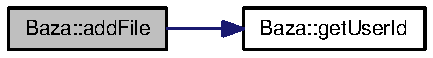
\includegraphics[width=122pt]{class_baza_f1bda4acd20e6fd00a35c43638e48956_cgraph}
\end{center}
\end{figure}
\hypertarget{class_baza_bef61cc396e46d347a47c75e9ef8dfde}{
\index{Baza@{Baza}!connect@{connect}}
\index{connect@{connect}!Baza@{Baza}}
\subsubsection[{connect}]{\setlength{\rightskip}{0pt plus 5cm}void Baza::connect (const char $\ast$ {\em server}, \/  const char $\ast$ {\em login}, \/  const char $\ast$ {\em pass}, \/  const char $\ast$ {\em db})}}
\label{class_baza_bef61cc396e46d347a47c75e9ef8dfde}


Łaczy się z bazą damych. 



Definicja w linii 3 pliku baza.cpp.

Here is the caller graph for this function:\nopagebreak
\begin{figure}[H]
\begin{center}
\leavevmode
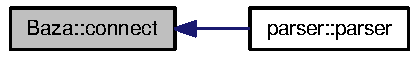
\includegraphics[width=118pt]{class_baza_bef61cc396e46d347a47c75e9ef8dfde_icgraph}
\end{center}
\end{figure}
\hypertarget{class_baza_a09b37e4665bd7b2f2b8b54f8120f5be}{
\index{Baza@{Baza}!get\_\-passwd@{get\_\-passwd}}
\index{get\_\-passwd@{get\_\-passwd}!Baza@{Baza}}
\subsubsection[{get\_\-passwd}]{\setlength{\rightskip}{0pt plus 5cm}std::string Baza::get\_\-passwd (std::string {\em login})}}
\label{class_baza_a09b37e4665bd7b2f2b8b54f8120f5be}


Pobiera hasło uzytkownika z bazy. 



Definicja w linii 19 pliku baza.cpp.\hypertarget{class_baza_1d1cfca062ab3117b2b97281df012823}{
\index{Baza@{Baza}!getFileInfo@{getFileInfo}}
\index{getFileInfo@{getFileInfo}!Baza@{Baza}}
\subsubsection[{getFileInfo}]{\setlength{\rightskip}{0pt plus 5cm}mysqlpp::StoreQueryResult Baza::getFileInfo (std::string {\em file}, \/  int {\em user\_\-id})}}
\label{class_baza_1d1cfca062ab3117b2b97281df012823}




Definicja w linii 131 pliku baza.cpp.\hypertarget{class_baza_e4a033a65cb585aa91c15fd8b8fde764}{
\index{Baza@{Baza}!getFileInfo@{getFileInfo}}
\index{getFileInfo@{getFileInfo}!Baza@{Baza}}
\subsubsection[{getFileInfo}]{\setlength{\rightskip}{0pt plus 5cm}mysqlpp::StoreQueryResult Baza::getFileInfo (std::string {\em file}, \/  std::string {\em user})}}
\label{class_baza_e4a033a65cb585aa91c15fd8b8fde764}


Podobnie jak getFilesList tylko ze pobiera informację o jednym pliku. 



Definicja w linii 115 pliku baza.cpp.

Oto graf wywołań dla tej funkcji:\nopagebreak
\begin{figure}[H]
\begin{center}
\leavevmode
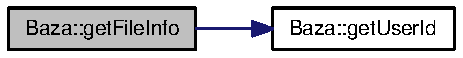
\includegraphics[width=129pt]{class_baza_e4a033a65cb585aa91c15fd8b8fde764_cgraph}
\end{center}
\end{figure}
\hypertarget{class_baza_2eace36725672b3a4ce639f91fe7d9bd}{
\index{Baza@{Baza}!getFilesList@{getFilesList}}
\index{getFilesList@{getFilesList}!Baza@{Baza}}
\subsubsection[{getFilesList}]{\setlength{\rightskip}{0pt plus 5cm}mysqlpp::StoreQueryResult Baza::getFilesList (std::string {\em user})}}
\label{class_baza_2eace36725672b3a4ce639f91fe7d9bd}


Najpierw wywołuje \hyperlink{class_baza_65054f08c8fd7c600f6c2fe2c7f61a43}{getUserId()} potem z id otrzymanym z tamtąd wywołuje \hyperlink{class_baza_02db3388d088212bd443ee39998b5cf8}{getFilesList(int user\_\-id)};. 

Zapytanie o listę plików uzytkownika o nazwie podanej w zmiennej user. 

Definicja w linii 61 pliku baza.cpp.

Oto graf wywołań dla tej funkcji:\nopagebreak
\begin{figure}[H]
\begin{center}
\leavevmode
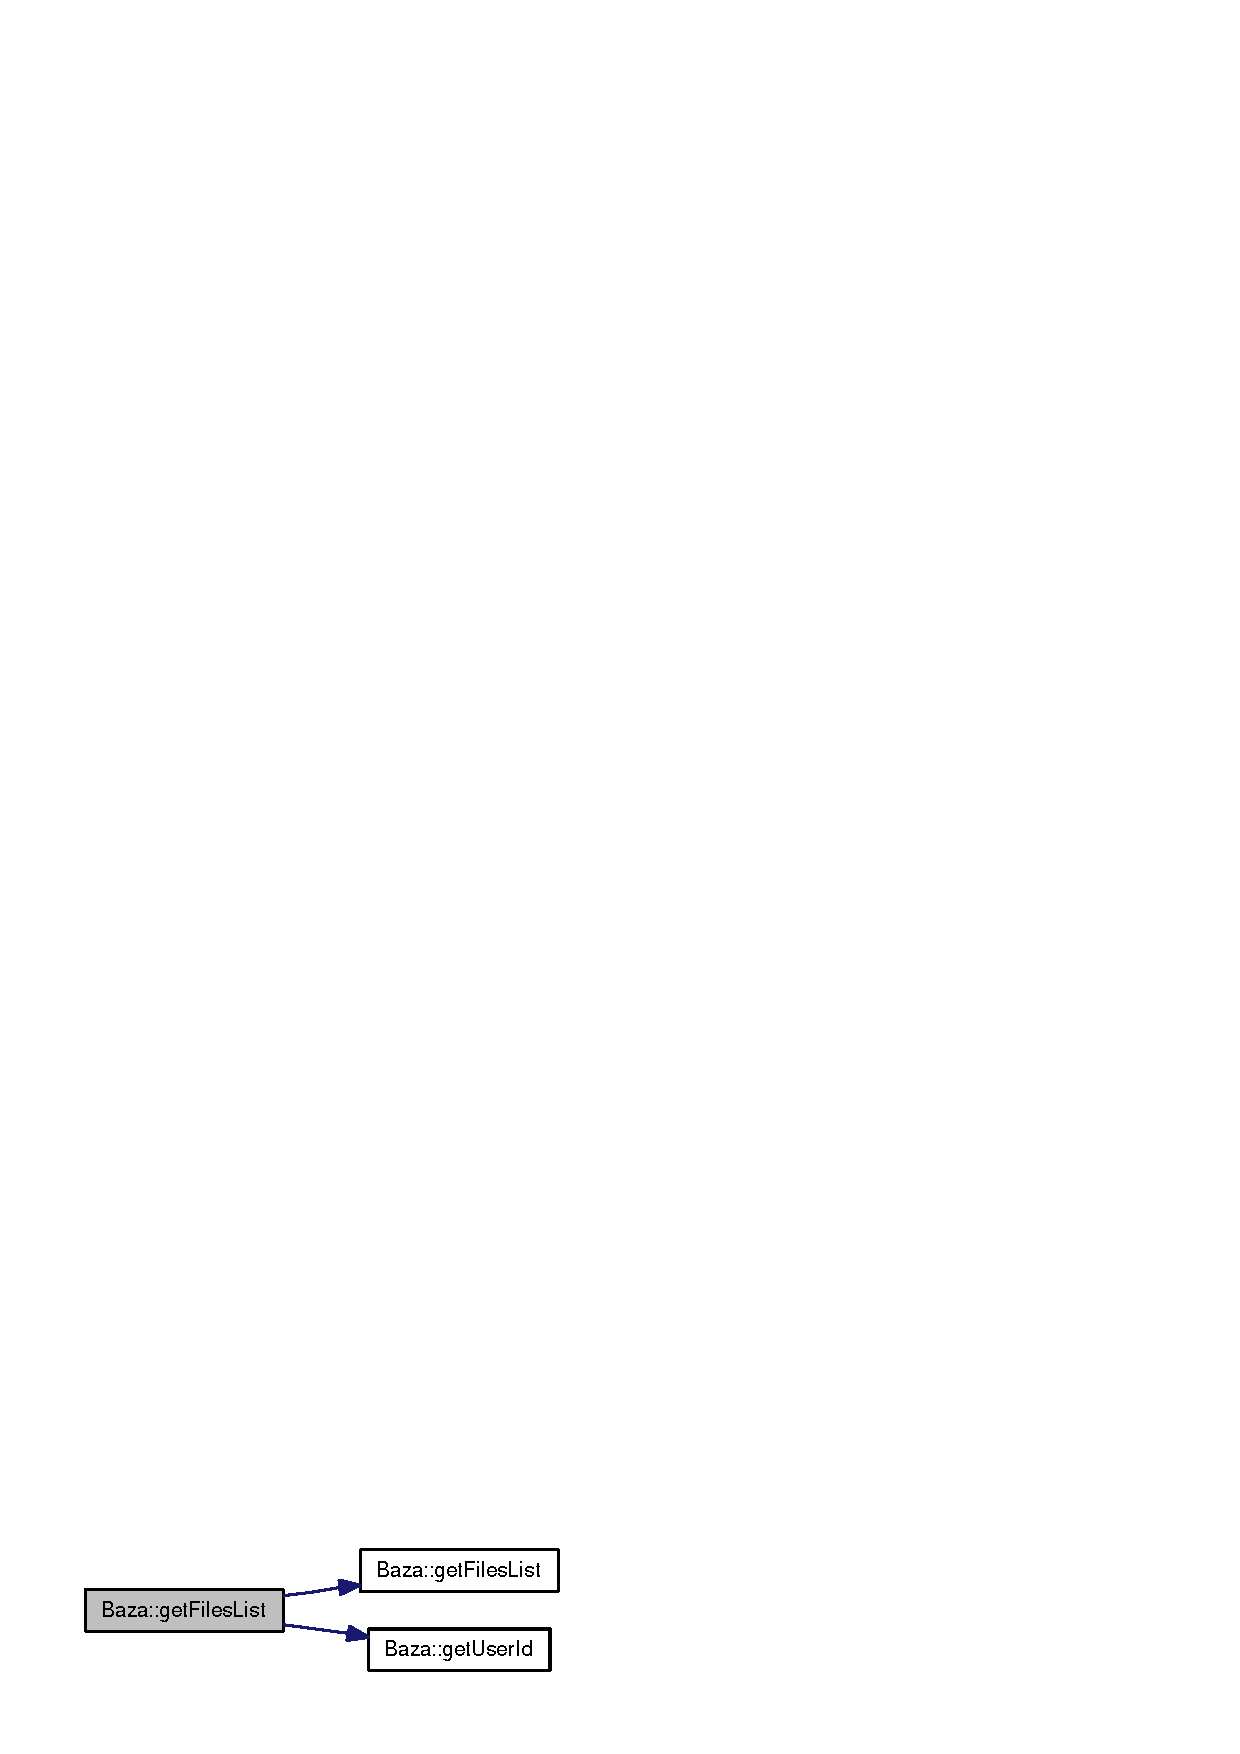
\includegraphics[width=136pt]{class_baza_2eace36725672b3a4ce639f91fe7d9bd_cgraph}
\end{center}
\end{figure}
\hypertarget{class_baza_02db3388d088212bd443ee39998b5cf8}{
\index{Baza@{Baza}!getFilesList@{getFilesList}}
\index{getFilesList@{getFilesList}!Baza@{Baza}}
\subsubsection[{getFilesList}]{\setlength{\rightskip}{0pt plus 5cm}mysqlpp::StoreQueryResult Baza::getFilesList (int {\em user\_\-id})}}
\label{class_baza_02db3388d088212bd443ee39998b5cf8}


Pobiera listę plików z bazy na podstawie ID uzytkownika. 

Zapytanie o listę plikow uzytkownika po id uzytkownika z bazy accounts\_\-konto. 

Definicja w linii 39 pliku baza.cpp.

Here is the caller graph for this function:\nopagebreak
\begin{figure}[H]
\begin{center}
\leavevmode
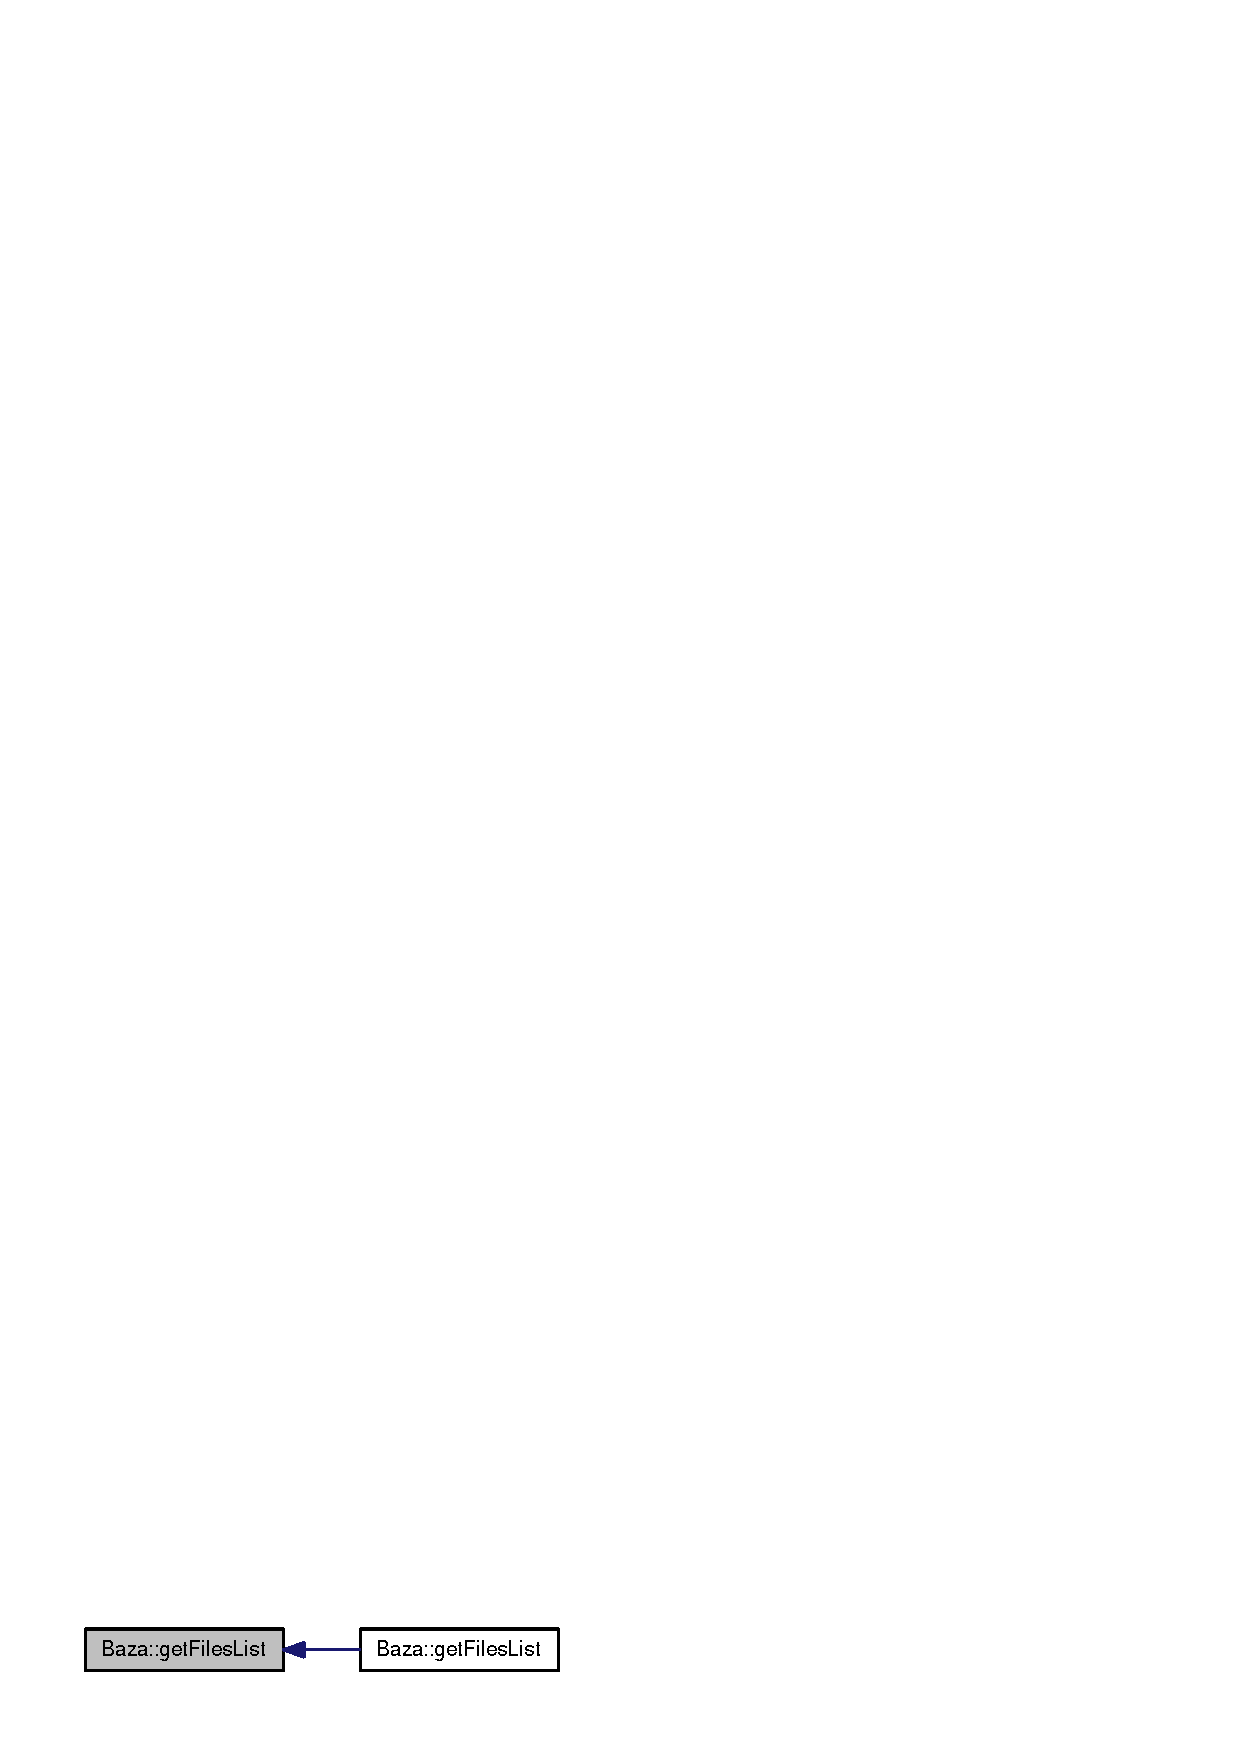
\includegraphics[width=136pt]{class_baza_02db3388d088212bd443ee39998b5cf8_icgraph}
\end{center}
\end{figure}
\hypertarget{class_baza_65054f08c8fd7c600f6c2fe2c7f61a43}{
\index{Baza@{Baza}!getUserId@{getUserId}}
\index{getUserId@{getUserId}!Baza@{Baza}}
\subsubsection[{getUserId}]{\setlength{\rightskip}{0pt plus 5cm}int Baza::getUserId (std::string {\em user})}}
\label{class_baza_65054f08c8fd7c600f6c2fe2c7f61a43}


Pobiera id uzytkownika 'user'. 

Zapytanie o ID uzytkownika o loginie 'user' ale nie o id z auth\_\-user tylko o id z accounts\_\-konto. 

Definicja w linii 79 pliku baza.cpp.

Here is the caller graph for this function:\nopagebreak
\begin{figure}[H]
\begin{center}
\leavevmode
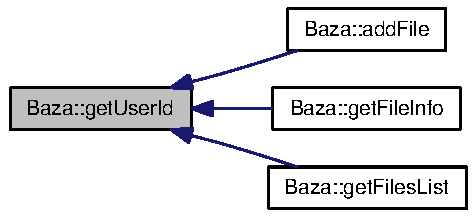
\includegraphics[width=132pt]{class_baza_65054f08c8fd7c600f6c2fe2c7f61a43_icgraph}
\end{center}
\end{figure}


Dokumentacja dla tej klasy została wygenerowana z plików:\begin{CompactItemize}
\item 
/home/pawel/Dokumenty/Uczelnia/grupappz/Source/Ass8-server/\hyperlink{baza_8hpp}{baza.hpp}\item 
/home/pawel/Dokumenty/Uczelnia/grupappz/Source/Ass8-server/\hyperlink{baza_8cpp}{baza.cpp}\end{CompactItemize}

\hypertarget{classparser}{
\section{Dokumentacja klasy parser}
\label{classparser}\index{parser@{parser}}
}
{\tt \#include $<$parser.hpp$>$}

Diagram współpracy dla parser:\nopagebreak
\begin{figure}[H]
\begin{center}
\leavevmode
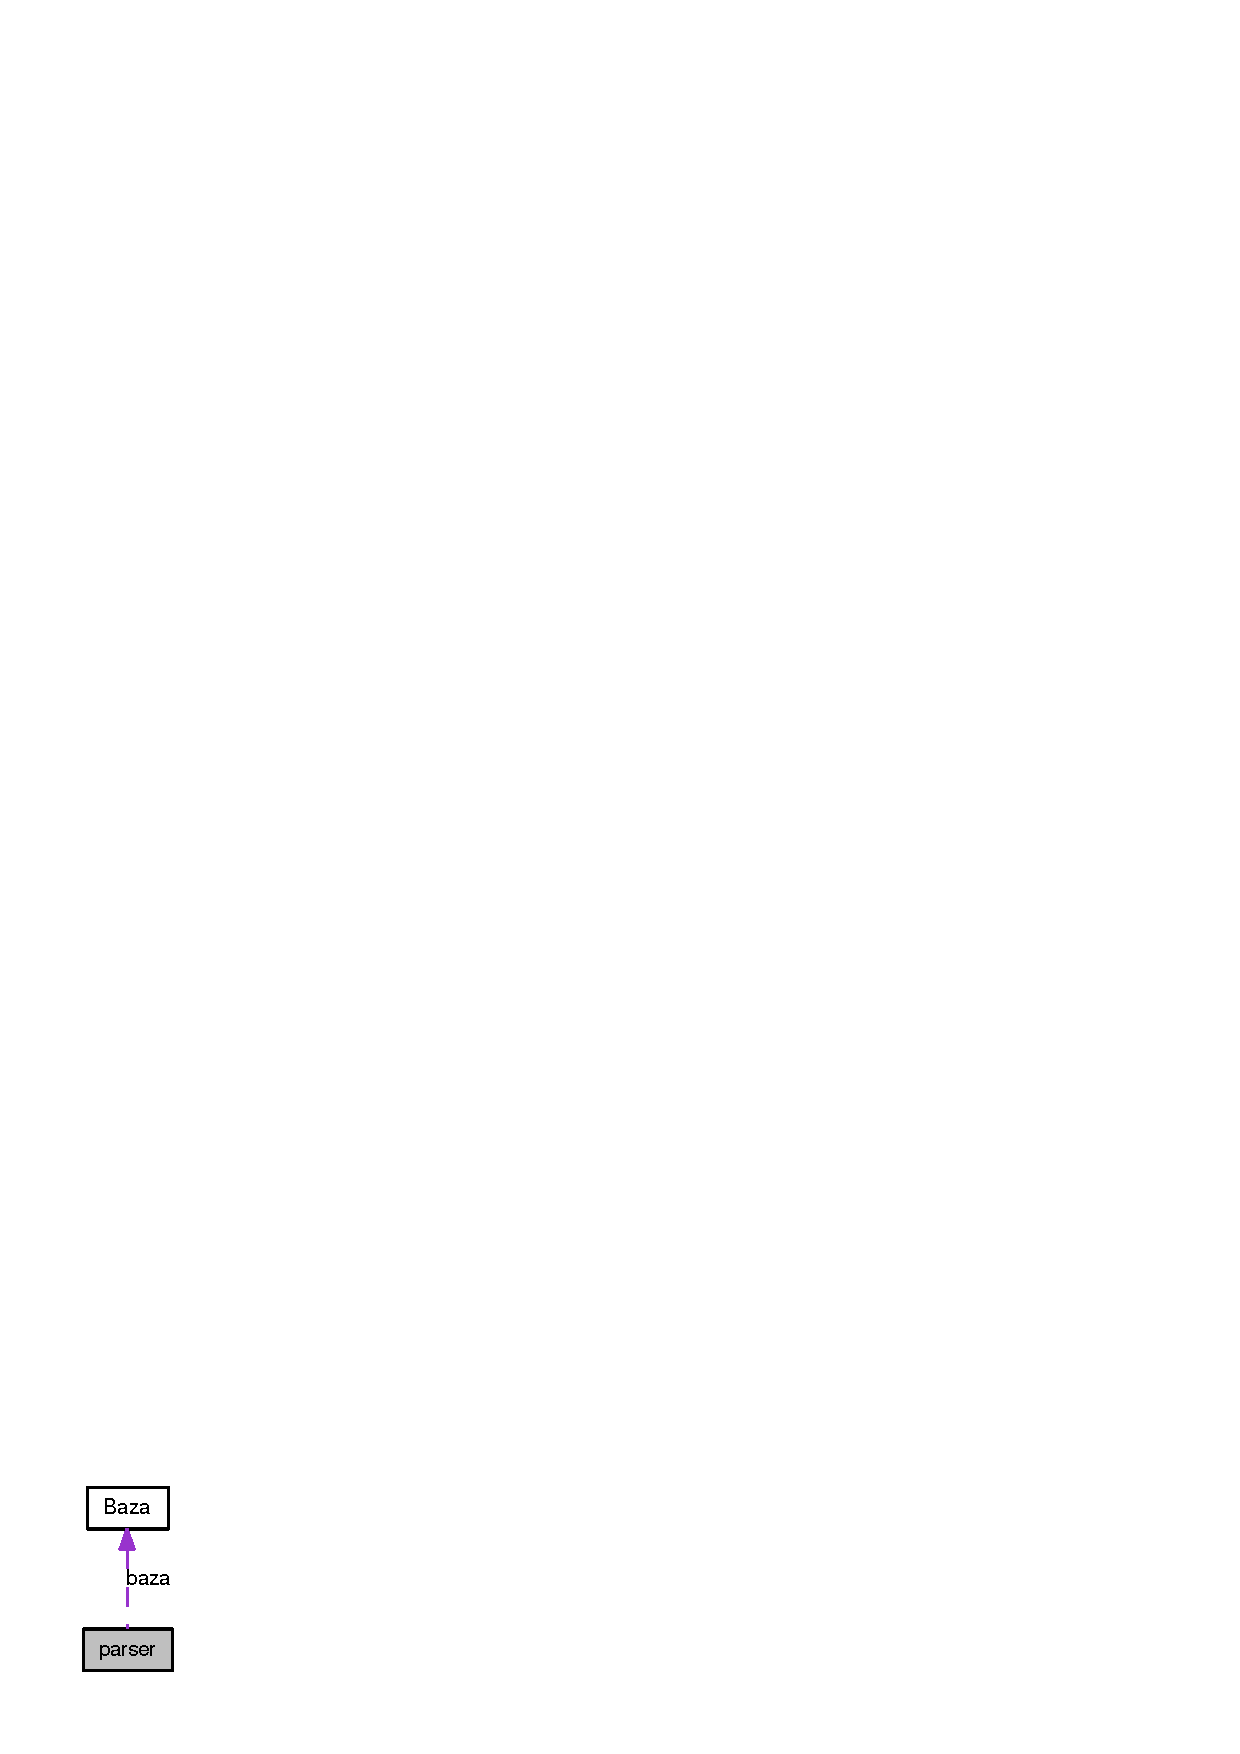
\includegraphics[width=86pt]{classparser__coll__graph}
\end{center}
\end{figure}
\subsection*{Metody publiczne}
\begin{CompactItemize}
\item 
\hyperlink{classparser_3a237071a3ab764cd61bc53df9dd4f46}{parser} (tcp::iostream \&stream, const char $\ast$server, const char $\ast$user, const char $\ast$pass, const char $\ast$db)
\item 
void \hyperlink{classparser_7793913f528921aa22c4b6cc259a0a14}{start} ()
\end{CompactItemize}


\subsection{Opis szczegółowy}


Definicja w linii 22 pliku parser.hpp.

\subsection{Dokumentacja konstruktora i destruktora}
\hypertarget{classparser_3a237071a3ab764cd61bc53df9dd4f46}{
\index{parser@{parser}!parser@{parser}}
\index{parser@{parser}!parser@{parser}}
\subsubsection[{parser}]{\setlength{\rightskip}{0pt plus 5cm}parser::parser (tcp::iostream \& {\em stream}, \/  const char $\ast$ {\em server}, \/  const char $\ast$ {\em user}, \/  const char $\ast$ {\em pass}, \/  const char $\ast$ {\em db})\hspace{0.3cm}{\tt  \mbox{[}inline\mbox{]}}}}
\label{classparser_3a237071a3ab764cd61bc53df9dd4f46}




Definicja w linii 71 pliku parser.hpp.

Oto graf wywołań dla tej funkcji:\nopagebreak
\begin{figure}[H]
\begin{center}
\leavevmode
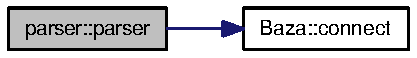
\includegraphics[width=118pt]{classparser_3a237071a3ab764cd61bc53df9dd4f46_cgraph}
\end{center}
\end{figure}


\subsection{Dokumentacja funkcji składowych}
\hypertarget{classparser_7793913f528921aa22c4b6cc259a0a14}{
\index{parser@{parser}!start@{start}}
\index{start@{start}!parser@{parser}}
\subsubsection[{start}]{\setlength{\rightskip}{0pt plus 5cm}void parser::start ()}}
\label{classparser_7793913f528921aa22c4b6cc259a0a14}




Here is the caller graph for this function:\nopagebreak
\begin{figure}[H]
\begin{center}
\leavevmode
\includegraphics[width=94pt]{classparser_7793913f528921aa22c4b6cc259a0a14_icgraph}
\end{center}
\end{figure}


Dokumentacja dla tej klasy została wygenerowana z plików:\begin{CompactItemize}
\item 
/home/pawel/Dokumenty/Uczelnia/grupappz/Source/Ass8-server/\hyperlink{parser_8hpp}{parser.hpp}\item 
/home/pawel/Dokumenty/Uczelnia/grupappz/Source/Ass8-server/\hyperlink{parser_8cpp}{parser.cpp}\end{CompactItemize}

\chapter{Dokumentacja plików}
\hypertarget{baza_8cpp}{
\section{Dokumentacja pliku /home/pawel/Dokumenty/Uczelnia/grupappz/Source/Ass8-server/baza.cpp}
\label{baza_8cpp}\index{/home/pawel/Dokumenty/Uczelnia/grupappz/Source/Ass8-server/baza.cpp@{/home/pawel/Dokumenty/Uczelnia/grupappz/Source/Ass8-server/baza.cpp}}
}
{\tt \#include \char`\"{}baza.hpp\char`\"{}}\par


Wykres zależności załączania dla baza.cpp:\nopagebreak
\begin{figure}[H]
\begin{center}
\leavevmode
\includegraphics[width=204pt]{baza_8cpp__incl}
\end{center}
\end{figure}

\hypertarget{baza_8hpp}{
\section{Dokumentacja pliku /home/pawel/Dokumenty/Uczelnia/grupappz/Source/Ass8-server/baza.hpp}
\label{baza_8hpp}\index{/home/pawel/Dokumenty/Uczelnia/grupappz/Source/Ass8-server/baza.hpp@{/home/pawel/Dokumenty/Uczelnia/grupappz/Source/Ass8-server/baza.hpp}}
}
{\tt \#include $<$string$>$}\par
{\tt \#include $<$mysql++.h$>$}\par
{\tt \#include $<$iostream$>$}\par
{\tt \#include $<$iomanip$>$}\par
{\tt \#include \char`\"{}debug.hpp\char`\"{}}\par


Wykres zależności załączania dla baza.hpp:\nopagebreak
\begin{figure}[H]
\begin{center}
\leavevmode
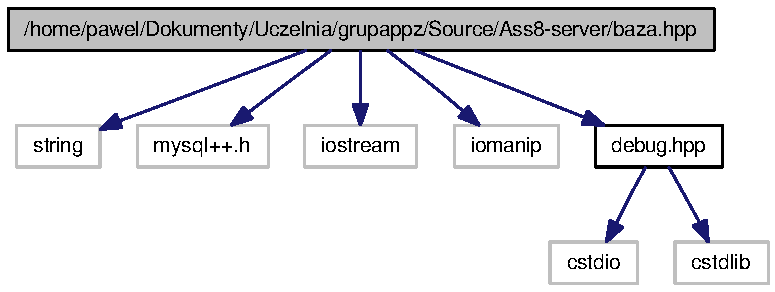
\includegraphics[width=204pt]{baza_8hpp__incl}
\end{center}
\end{figure}


Ten wykres pokazuje, które pliki bezpośrednio lub pośrednio załączają ten plik:\nopagebreak
\begin{figure}[H]
\begin{center}
\leavevmode
\includegraphics[width=420pt]{baza_8hpp__dep__incl}
\end{center}
\end{figure}
\subsection*{Komponenty}
\begin{CompactItemize}
\item 
class \hyperlink{class_baza}{Baza}
\end{CompactItemize}

\hypertarget{debug_8hpp}{
\section{Dokumentacja pliku /home/pawel/Dokumenty/Uczelnia/grupappz/Source/Ass8-server/debug.hpp}
\label{debug_8hpp}\index{/home/pawel/Dokumenty/Uczelnia/grupappz/Source/Ass8-server/debug.hpp@{/home/pawel/Dokumenty/Uczelnia/grupappz/Source/Ass8-server/debug.hpp}}
}
{\tt \#include $<$cstdio$>$}\par
{\tt \#include $<$cstdlib$>$}\par


Wykres zależności załączania dla debug.hpp:\nopagebreak
\begin{figure}[H]
\begin{center}
\leavevmode
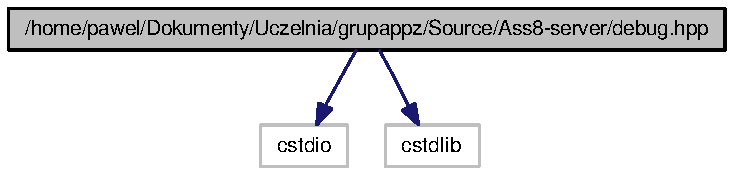
\includegraphics[width=194pt]{debug_8hpp__incl}
\end{center}
\end{figure}


Ten wykres pokazuje, które pliki bezpośrednio lub pośrednio załączają ten plik:\nopagebreak
\begin{figure}[H]
\begin{center}
\leavevmode
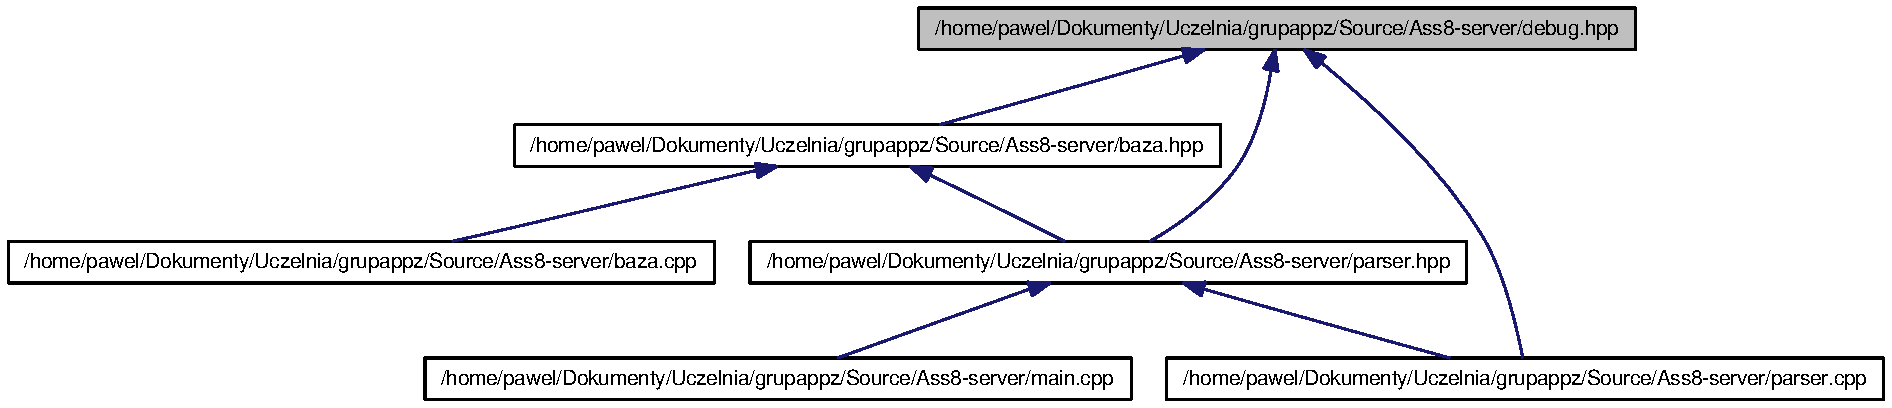
\includegraphics[width=420pt]{debug_8hpp__dep__incl}
\end{center}
\end{figure}
\subsection*{Definicje}
\begin{CompactItemize}
\item 
\#define \hyperlink{debug_8hpp_d72dbcf6d0153db1b8d8a58001feed83}{DEBUG}
\item 
\#define \hyperlink{debug_8hpp_21ad5938437ed6d1865dd14c8d1871bc}{deb}(arg, arg2)~fprintf(stderr,(arg),(arg2));
\item 
\#define \hyperlink{debug_8hpp_5bdec07ba0f5f220bcb40d5258725d95}{line}~fprintf(stderr,\char`\"{}I: \%s : \%d$\backslash$n\char`\"{},\_\-\_\-FILE\_\-\_\-,\_\-\_\-LINE\_\-\_\-);
\item 
\#define \hyperlink{debug_8hpp_b3fdd01cf4ecc9316aa5051f88e36af2}{Eline}(arg)~fprintf(stderr,\char`\"{}E: \%s : \%d : \%s $\backslash$n\char`\"{},\_\-\_\-FILE\_\-\_\-,\_\-\_\-LINE\_\-\_\-,arg);
\item 
\#define \hyperlink{debug_8hpp_66e7745144eb47a4111a0c2b5f66d6ac}{Eline2}(arg, arg2)~fprintf(stderr,\char`\"{}E: \%s : \%d : \%s \%s$\backslash$n\char`\"{},\_\-\_\-FILE\_\-\_\-,\_\-\_\-LINE\_\-\_\-,arg,arg2);
\item 
\#define \hyperlink{debug_8hpp_590af51ecfed28223c4e6ce02994241a}{info}(arg)~fprintf(stderr,\char`\"{}I: \%s : \%d : \%s$\backslash$n\char`\"{},\_\-\_\-FILE\_\-\_\-,\_\-\_\-LINE\_\-\_\-,arg);
\item 
\#define \hyperlink{debug_8hpp_51633d6d15647d74f756bcf969fc70ae}{info2}(arg, arg2)~fprintf(stderr,\char`\"{}I: \%s : \%d : \%s =$>$ \%s$\backslash$n\char`\"{},\_\-\_\-FILE\_\-\_\-,\_\-\_\-LINE\_\-\_\-,arg,arg2);
\end{CompactItemize}


\subsection{Dokumentacja definicji}
\hypertarget{debug_8hpp_21ad5938437ed6d1865dd14c8d1871bc}{
\index{debug.hpp@{debug.hpp}!deb@{deb}}
\index{deb@{deb}!debug.hpp@{debug.hpp}}
\subsubsection[{deb}]{\setlength{\rightskip}{0pt plus 5cm}\#define deb(arg, \/  arg2)~fprintf(stderr,(arg),(arg2));}}
\label{debug_8hpp_21ad5938437ed6d1865dd14c8d1871bc}




Definicja w linii 7 pliku debug.hpp.\hypertarget{debug_8hpp_d72dbcf6d0153db1b8d8a58001feed83}{
\index{debug.hpp@{debug.hpp}!DEBUG@{DEBUG}}
\index{DEBUG@{DEBUG}!debug.hpp@{debug.hpp}}
\subsubsection[{DEBUG}]{\setlength{\rightskip}{0pt plus 5cm}\#define DEBUG}}
\label{debug_8hpp_d72dbcf6d0153db1b8d8a58001feed83}




Definicja w linii 5 pliku debug.hpp.\hypertarget{debug_8hpp_b3fdd01cf4ecc9316aa5051f88e36af2}{
\index{debug.hpp@{debug.hpp}!Eline@{Eline}}
\index{Eline@{Eline}!debug.hpp@{debug.hpp}}
\subsubsection[{Eline}]{\setlength{\rightskip}{0pt plus 5cm}\#define Eline(arg)~fprintf(stderr,\char`\"{}E: \%s : \%d : \%s $\backslash$n\char`\"{},\_\-\_\-FILE\_\-\_\-,\_\-\_\-LINE\_\-\_\-,arg);}}
\label{debug_8hpp_b3fdd01cf4ecc9316aa5051f88e36af2}




Definicja w linii 9 pliku debug.hpp.\hypertarget{debug_8hpp_66e7745144eb47a4111a0c2b5f66d6ac}{
\index{debug.hpp@{debug.hpp}!Eline2@{Eline2}}
\index{Eline2@{Eline2}!debug.hpp@{debug.hpp}}
\subsubsection[{Eline2}]{\setlength{\rightskip}{0pt plus 5cm}\#define Eline2(arg, \/  arg2)~fprintf(stderr,\char`\"{}E: \%s : \%d : \%s \%s$\backslash$n\char`\"{},\_\-\_\-FILE\_\-\_\-,\_\-\_\-LINE\_\-\_\-,arg,arg2);}}
\label{debug_8hpp_66e7745144eb47a4111a0c2b5f66d6ac}




Definicja w linii 10 pliku debug.hpp.\hypertarget{debug_8hpp_590af51ecfed28223c4e6ce02994241a}{
\index{debug.hpp@{debug.hpp}!info@{info}}
\index{info@{info}!debug.hpp@{debug.hpp}}
\subsubsection[{info}]{\setlength{\rightskip}{0pt plus 5cm}\#define info(arg)~fprintf(stderr,\char`\"{}I: \%s : \%d : \%s$\backslash$n\char`\"{},\_\-\_\-FILE\_\-\_\-,\_\-\_\-LINE\_\-\_\-,arg);}}
\label{debug_8hpp_590af51ecfed28223c4e6ce02994241a}




Definicja w linii 11 pliku debug.hpp.\hypertarget{debug_8hpp_51633d6d15647d74f756bcf969fc70ae}{
\index{debug.hpp@{debug.hpp}!info2@{info2}}
\index{info2@{info2}!debug.hpp@{debug.hpp}}
\subsubsection[{info2}]{\setlength{\rightskip}{0pt plus 5cm}\#define info2(arg, \/  arg2)~fprintf(stderr,\char`\"{}I: \%s : \%d : \%s =$>$ \%s$\backslash$n\char`\"{},\_\-\_\-FILE\_\-\_\-,\_\-\_\-LINE\_\-\_\-,arg,arg2);}}
\label{debug_8hpp_51633d6d15647d74f756bcf969fc70ae}




Definicja w linii 12 pliku debug.hpp.\hypertarget{debug_8hpp_5bdec07ba0f5f220bcb40d5258725d95}{
\index{debug.hpp@{debug.hpp}!line@{line}}
\index{line@{line}!debug.hpp@{debug.hpp}}
\subsubsection[{line}]{\setlength{\rightskip}{0pt plus 5cm}\#define line~fprintf(stderr,\char`\"{}I: \%s : \%d$\backslash$n\char`\"{},\_\-\_\-FILE\_\-\_\-,\_\-\_\-LINE\_\-\_\-);}}
\label{debug_8hpp_5bdec07ba0f5f220bcb40d5258725d95}




Definicja w linii 8 pliku debug.hpp.
\hypertarget{main_8cpp}{
\section{Dokumentacja pliku /home/pawel/Dokumenty/Uczelnia/grupappz/Source/Ass8-server/main.cpp}
\label{main_8cpp}\index{/home/pawel/Dokumenty/Uczelnia/grupappz/Source/Ass8-server/main.cpp@{/home/pawel/Dokumenty/Uczelnia/grupappz/Source/Ass8-server/main.cpp}}
}
{\tt \#include $<$iostream$>$}\par
{\tt \#include $<$string$>$}\par
{\tt \#include $<$cstdio$>$}\par
{\tt \#include $<$cstdlib$>$}\par
{\tt \#include $<$sys/types.h$>$}\par
{\tt \#include $<$unistd.h$>$}\par
{\tt \#include $<$sys/wait.h$>$}\par
{\tt \#include $<$boost/asio.hpp$>$}\par
{\tt \#include $<$boost/thread/thread.hpp$>$}\par
{\tt \#include $<$boost/bind.hpp$>$}\par
{\tt \#include \char`\"{}version.h\char`\"{}}\par
{\tt \#include \char`\"{}parser.hpp\char`\"{}}\par


Wykres zależności załączania dla main.cpp:\nopagebreak
\begin{figure}[H]
\begin{center}
\leavevmode
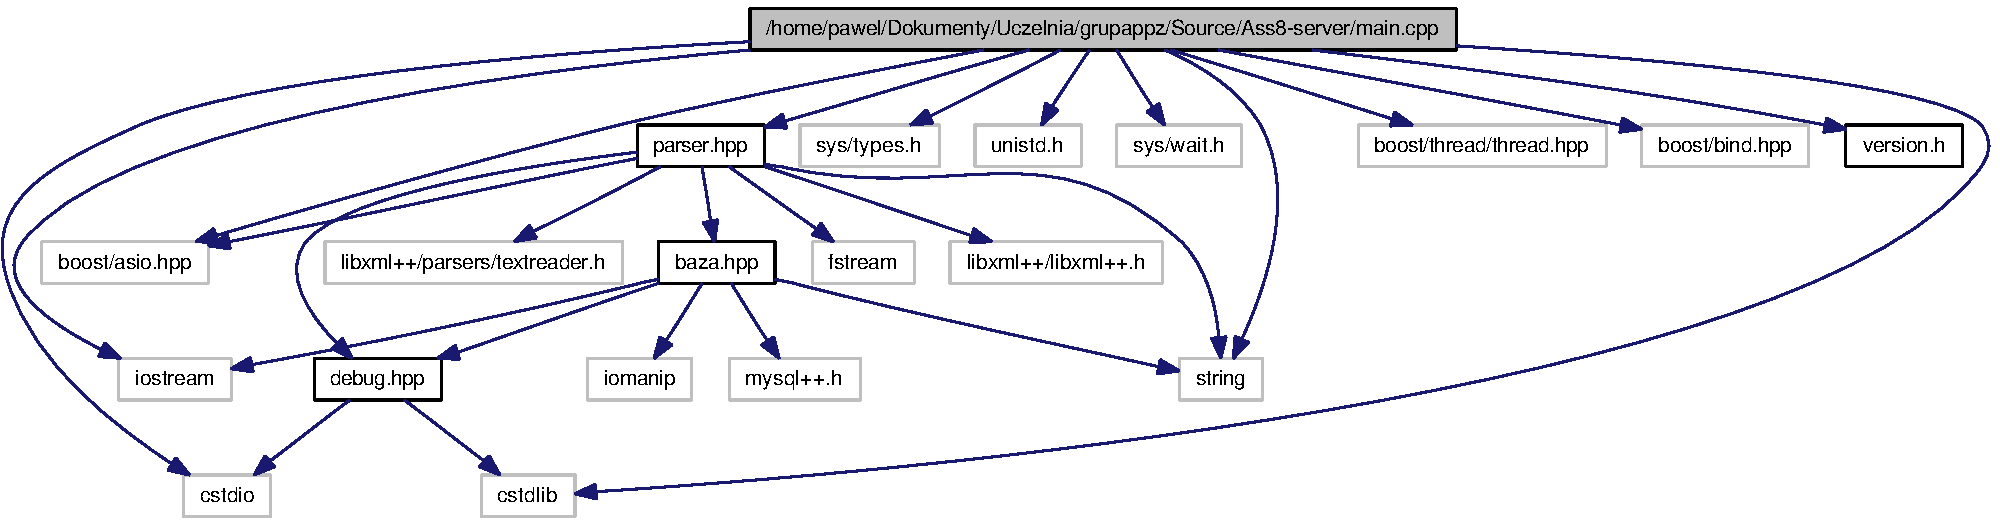
\includegraphics[width=420pt]{main_8cpp__incl}
\end{center}
\end{figure}
\subsection*{Funkcje}
\begin{CompactItemize}
\item 
int \hyperlink{main_8cpp_0ddf1224851353fc92bfbff6f499fa97}{main} (int argc, char $\ast$argv\mbox{[}$\,$\mbox{]})
\end{CompactItemize}


\subsection{Dokumentacja funkcji}
\hypertarget{main_8cpp_0ddf1224851353fc92bfbff6f499fa97}{
\index{main.cpp@{main.cpp}!main@{main}}
\index{main@{main}!main.cpp@{main.cpp}}
\subsubsection[{main}]{\setlength{\rightskip}{0pt plus 5cm}int main (int {\em argc}, \/  char $\ast$ {\em argv}\mbox{[}$\,$\mbox{]})}}
\label{main_8cpp_0ddf1224851353fc92bfbff6f499fa97}




Zmienna przechowująca port na którym serwer nasłucuje

Zmienne przechowujące parametry podłączenia do bazy danych

Zmienna przechowująca nazwę bazy w bazie danych

Jeżeli jest mniej niż 5 argumentów

To kończymy program

Potrzebne do połączenia z klientem

Potrzebne do połączenia z klientem

Potrzebne do połączenia z klientem

Watek ktory bedzie usuwal skonczone forki

Nieskonczona pętla

Wyjście/Wejście socketa

utworzenie parsera w forku (dla każdego klienta jeden taki jest tworzony); 

Definicja w linii 30 pliku main.cpp.

Oto graf wywołań dla tej funkcji:\nopagebreak
\begin{figure}[H]
\begin{center}
\leavevmode
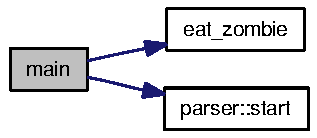
\includegraphics[width=94pt]{main_8cpp_0ddf1224851353fc92bfbff6f499fa97_cgraph}
\end{center}
\end{figure}

\hypertarget{parser_8cpp}{
\section{Dokumentacja pliku /home/pawel/Dokumenty/Uczelnia/grupappz/Source/Ass8-server/parser.cpp}
\label{parser_8cpp}\index{/home/pawel/Dokumenty/Uczelnia/grupappz/Source/Ass8-server/parser.cpp@{/home/pawel/Dokumenty/Uczelnia/grupappz/Source/Ass8-server/parser.cpp}}
}
{\tt \#include $<$iostream$>$}\par
{\tt \#include $<$string$>$}\par
{\tt \#include $<$cstdlib$>$}\par
{\tt \#include $<$cstdio$>$}\par
{\tt \#include $<$vector$>$}\par
{\tt \#include $<$sys/types.h$>$}\par
{\tt \#include $<$unistd.h$>$}\par
{\tt \#include $<$sys/wait.h$>$}\par
{\tt \#include \char`\"{}version.h\char`\"{}}\par
{\tt \#include \char`\"{}parser.hpp\char`\"{}}\par
{\tt \#include \char`\"{}xml.hpp\char`\"{}}\par
{\tt \#include \char`\"{}debug.hpp\char`\"{}}\par


Wykres zależności załączania dla parser.cpp:\nopagebreak
\begin{figure}[H]
\begin{center}
\leavevmode
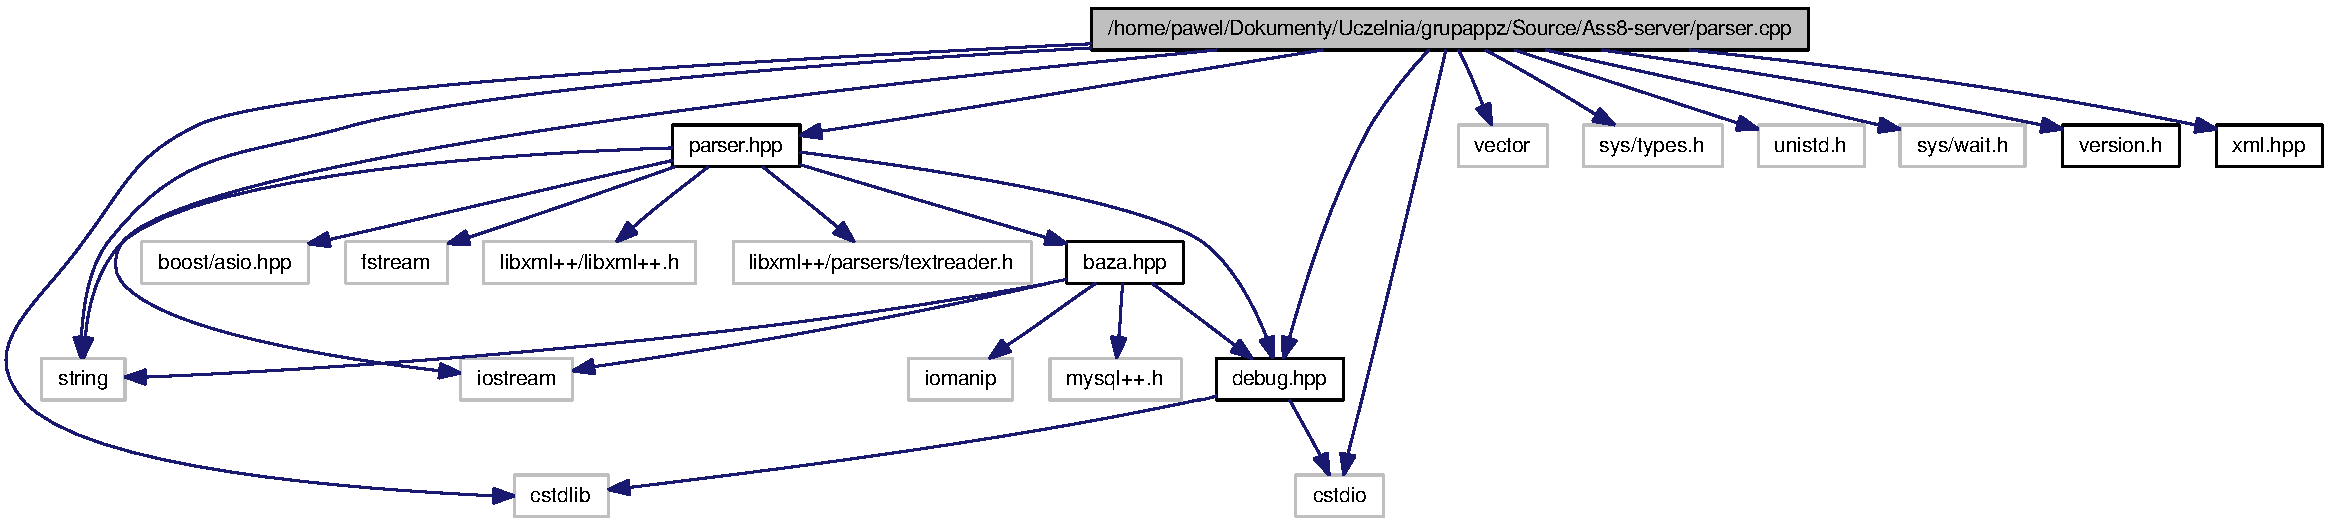
\includegraphics[width=420pt]{parser_8cpp__incl}
\end{center}
\end{figure}

\hypertarget{parser_8hpp}{
\section{Dokumentacja pliku /home/pawel/Dokumenty/Uczelnia/grupappz/Source/Ass8-server/parser.hpp}
\label{parser_8hpp}\index{/home/pawel/Dokumenty/Uczelnia/grupappz/Source/Ass8-server/parser.hpp@{/home/pawel/Dokumenty/Uczelnia/grupappz/Source/Ass8-server/parser.hpp}}
}
{\tt \#include $<$boost/asio.hpp$>$}\par
{\tt \#include $<$string$>$}\par
{\tt \#include $<$fstream$>$}\par
{\tt \#include $<$libxml++/libxml++.h$>$}\par
{\tt \#include $<$libxml++/parsers/textreader.h$>$}\par
{\tt \#include \char`\"{}baza.hpp\char`\"{}}\par
{\tt \#include \char`\"{}debug.hpp\char`\"{}}\par


Wykres zależności załączania dla parser.hpp:\nopagebreak
\begin{figure}[H]
\begin{center}
\leavevmode
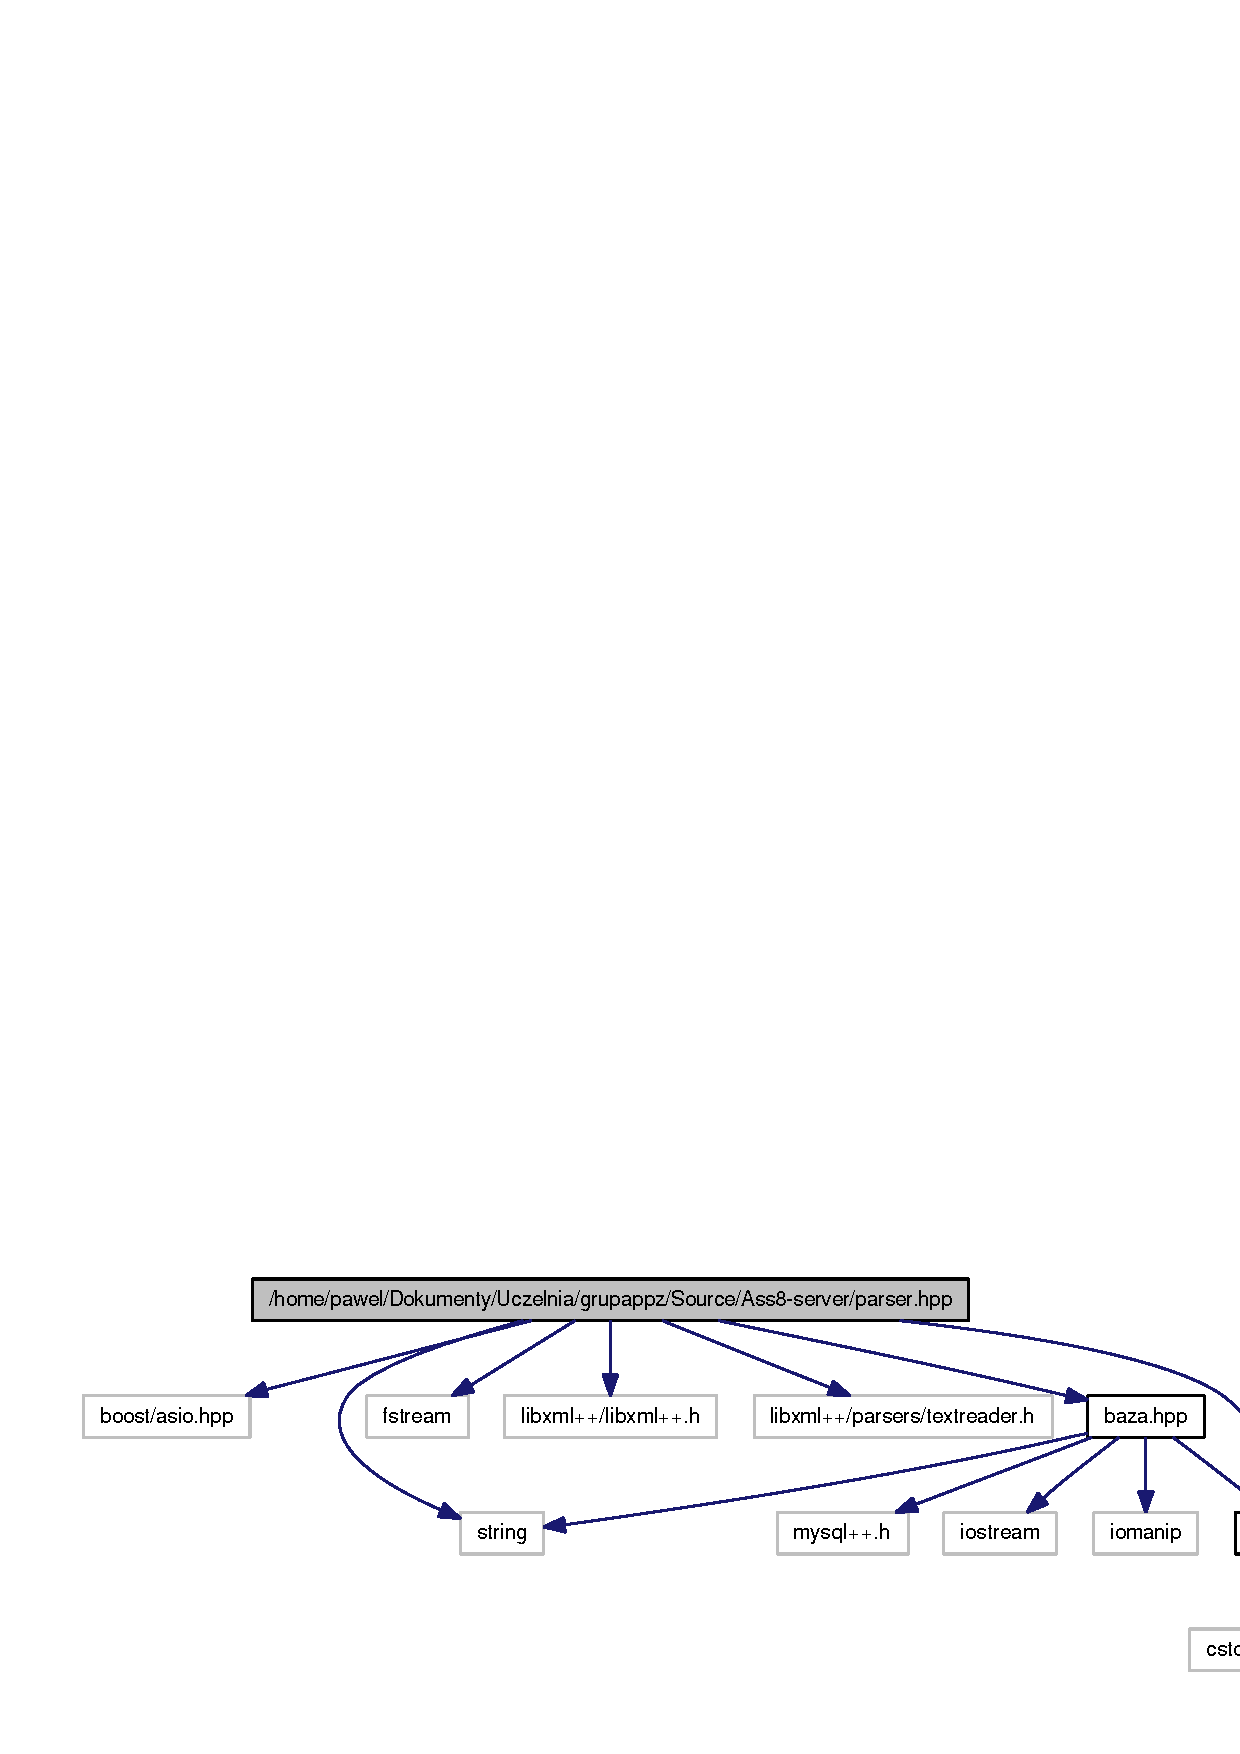
\includegraphics[width=339pt]{parser_8hpp__incl}
\end{center}
\end{figure}


Ten wykres pokazuje, które pliki bezpośrednio lub pośrednio załączają ten plik:\nopagebreak
\begin{figure}[H]
\begin{center}
\leavevmode
\includegraphics[width=372pt]{parser_8hpp__dep__incl}
\end{center}
\end{figure}
\subsection*{Komponenty}
\begin{CompactItemize}
\item 
class \hyperlink{classparser}{parser}
\end{CompactItemize}
\subsection*{Definicje}
\begin{CompactItemize}
\item 
\#define \hyperlink{parser_8hpp_eca034f67218340ecb2261a22c2f3dcd}{BUFSIZE}~1024
\item 
\#define \hyperlink{parser_8hpp_b46db07bcc5d1bb3dbc73f7be2592ee0}{BUFSIZE2}~1024$\ast$2
\end{CompactItemize}
\subsection*{Funkcje}
\begin{CompactItemize}
\item 
void \hyperlink{parser_8hpp_6c724feff242ad0cd599cdd458f73199}{eat\_\-zombie} ()
\end{CompactItemize}


\subsection{Dokumentacja definicji}
\hypertarget{parser_8hpp_eca034f67218340ecb2261a22c2f3dcd}{
\index{parser.hpp@{parser.hpp}!BUFSIZE@{BUFSIZE}}
\index{BUFSIZE@{BUFSIZE}!parser.hpp@{parser.hpp}}
\subsubsection[{BUFSIZE}]{\setlength{\rightskip}{0pt plus 5cm}\#define BUFSIZE~1024}}
\label{parser_8hpp_eca034f67218340ecb2261a22c2f3dcd}




Definicja w linii 19 pliku parser.hpp.\hypertarget{parser_8hpp_b46db07bcc5d1bb3dbc73f7be2592ee0}{
\index{parser.hpp@{parser.hpp}!BUFSIZE2@{BUFSIZE2}}
\index{BUFSIZE2@{BUFSIZE2}!parser.hpp@{parser.hpp}}
\subsubsection[{BUFSIZE2}]{\setlength{\rightskip}{0pt plus 5cm}\#define BUFSIZE2~1024$\ast$2}}
\label{parser_8hpp_b46db07bcc5d1bb3dbc73f7be2592ee0}




Definicja w linii 20 pliku parser.hpp.

\subsection{Dokumentacja funkcji}
\hypertarget{parser_8hpp_6c724feff242ad0cd599cdd458f73199}{
\index{parser.hpp@{parser.hpp}!eat\_\-zombie@{eat\_\-zombie}}
\index{eat\_\-zombie@{eat\_\-zombie}!parser.hpp@{parser.hpp}}
\subsubsection[{eat\_\-zombie}]{\setlength{\rightskip}{0pt plus 5cm}void eat\_\-zombie ()}}
\label{parser_8hpp_6c724feff242ad0cd599cdd458f73199}




Here is the caller graph for this function:\nopagebreak
\begin{figure}[H]
\begin{center}
\leavevmode
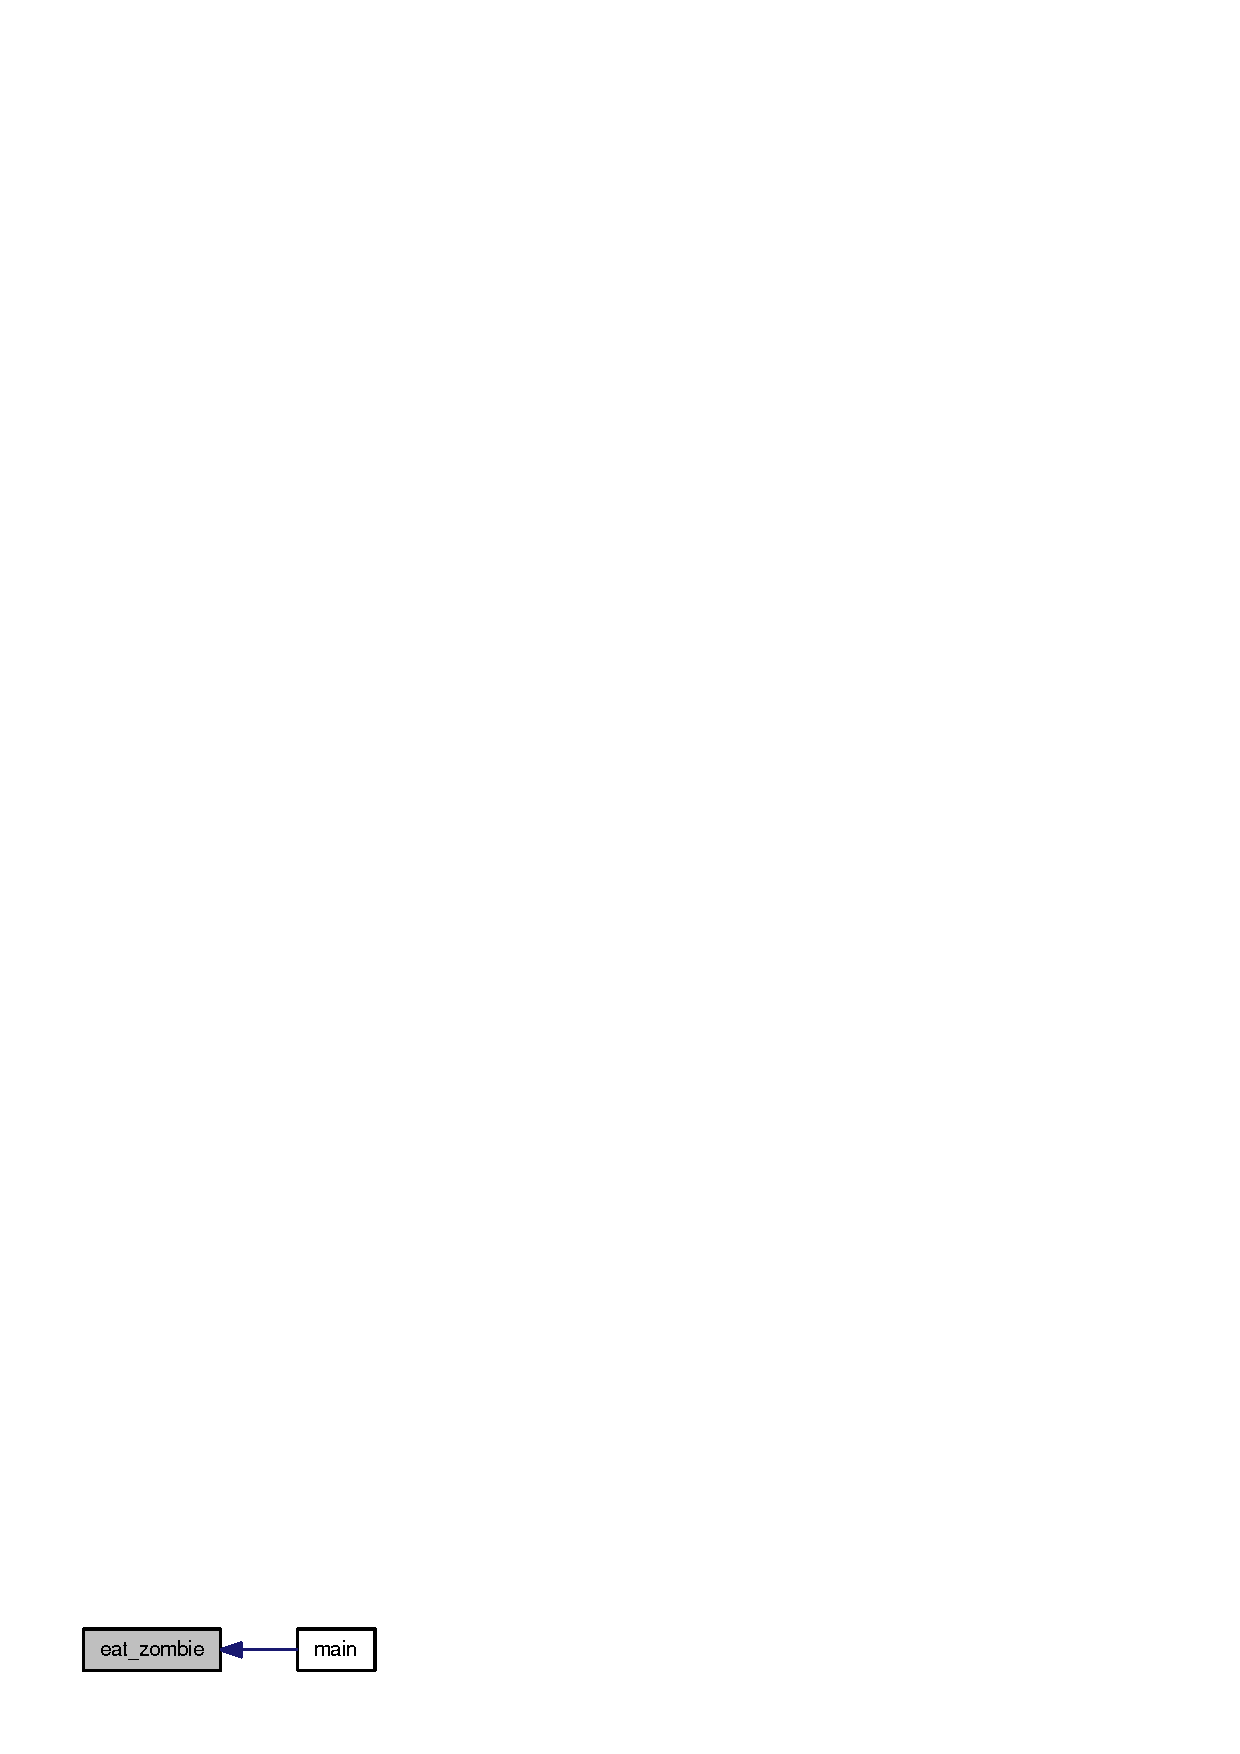
\includegraphics[width=92pt]{parser_8hpp_6c724feff242ad0cd599cdd458f73199_icgraph}
\end{center}
\end{figure}

\hypertarget{server_8hpp}{
\section{Dokumentacja pliku /home/pawel/Dokumenty/Uczelnia/grupappz/Source/Ass8-server/server.hpp}
\label{server_8hpp}\index{/home/pawel/Dokumenty/Uczelnia/grupappz/Source/Ass8-server/server.hpp@{/home/pawel/Dokumenty/Uczelnia/grupappz/Source/Ass8-server/server.hpp}}
}

\hypertarget{version_8h}{
\section{Dokumentacja pliku /home/pawel/Dokumenty/Uczelnia/grupappz/Source/Ass8-server/version.h}
\label{version_8h}\index{/home/pawel/Dokumenty/Uczelnia/grupappz/Source/Ass8-server/version.h@{/home/pawel/Dokumenty/Uczelnia/grupappz/Source/Ass8-server/version.h}}
}


Ten wykres pokazuje, które pliki bezpośrednio lub pośrednio załączają ten plik:\nopagebreak
\begin{figure}[H]
\begin{center}
\leavevmode
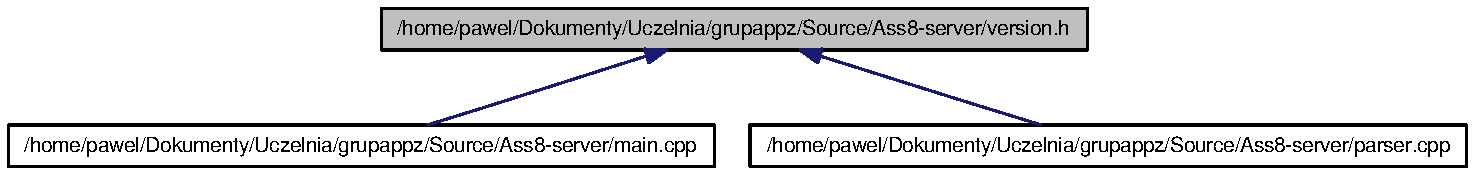
\includegraphics[width=372pt]{version_8h__dep__incl}
\end{center}
\end{figure}
\subsection*{Przestrzenie nazw}
\begin{CompactItemize}
\item 
namespace \hyperlink{namespace_auto_version}{AutoVersion}
\end{CompactItemize}
\subsection*{Definicje}
\begin{CompactItemize}
\item 
\#define \hyperlink{version_8h_0e86d046ea87587e402d375c6b0927c6}{RC\_\-FILEVERSION}~0,3,16,112
\item 
\#define \hyperlink{version_8h_4763e81d3c29ec0fab79225d3ec3f1a2}{RC\_\-FILEVERSION\_\-STRING}~\char`\"{}0, 3, 16, 112$\backslash$0\char`\"{}
\end{CompactItemize}


\subsection{Dokumentacja definicji}
\hypertarget{version_8h_0e86d046ea87587e402d375c6b0927c6}{
\index{version.h@{version.h}!RC\_\-FILEVERSION@{RC\_\-FILEVERSION}}
\index{RC\_\-FILEVERSION@{RC\_\-FILEVERSION}!version.h@{version.h}}
\subsubsection[{RC\_\-FILEVERSION}]{\setlength{\rightskip}{0pt plus 5cm}\#define RC\_\-FILEVERSION~0,3,16,112}}
\label{version_8h_0e86d046ea87587e402d375c6b0927c6}




Definicja w linii 24 pliku version.h.\hypertarget{version_8h_4763e81d3c29ec0fab79225d3ec3f1a2}{
\index{version.h@{version.h}!RC\_\-FILEVERSION\_\-STRING@{RC\_\-FILEVERSION\_\-STRING}}
\index{RC\_\-FILEVERSION\_\-STRING@{RC\_\-FILEVERSION\_\-STRING}!version.h@{version.h}}
\subsubsection[{RC\_\-FILEVERSION\_\-STRING}]{\setlength{\rightskip}{0pt plus 5cm}\#define RC\_\-FILEVERSION\_\-STRING~\char`\"{}0, 3, 16, 112$\backslash$0\char`\"{}}}
\label{version_8h_4763e81d3c29ec0fab79225d3ec3f1a2}




Definicja w linii 25 pliku version.h.
\hypertarget{xml_8hpp}{
\section{Dokumentacja pliku /home/pawel/Dokumenty/Uczelnia/grupappz/Source/Ass8-server/xml.hpp}
\label{xml_8hpp}\index{/home/pawel/Dokumenty/Uczelnia/grupappz/Source/Ass8-server/xml.hpp@{/home/pawel/Dokumenty/Uczelnia/grupappz/Source/Ass8-server/xml.hpp}}
}


Ten wykres pokazuje, które pliki bezpośrednio lub pośrednio załączają ten plik:\nopagebreak
\begin{figure}[H]
\begin{center}
\leavevmode
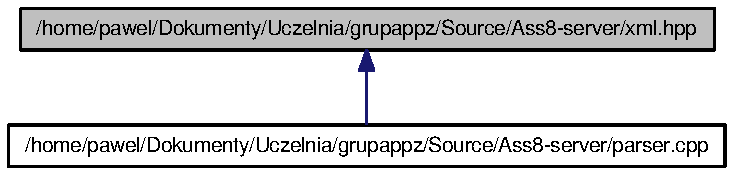
\includegraphics[width=194pt]{xml_8hpp__dep__incl}
\end{center}
\end{figure}

\printindex
\end{document}
